\documentclass[11pt,letterpaper]{article}
\usepackage[margin=1.0in]{geometry}
\usepackage[utf8]{inputenc}
\usepackage{cite}
\usepackage{amsmath}
\usepackage{amsfonts}
\usepackage{amssymb}
\usepackage{makeidx}
\usepackage{graphicx}
\usepackage{hyperref}
\setlength\parindent{0pt}

\author{STUDENT NAME}
\title{Lab3: Step response of a first order system}

\begin{document}

\maketitle

\section{Objectives}

The objective of this lab is to understand the functioning of an RC network, and its responses to common inputs such as the step and impulse.

\section{Introduction}

Given is a simple electrical first order system:
\begin{figure}
\centering
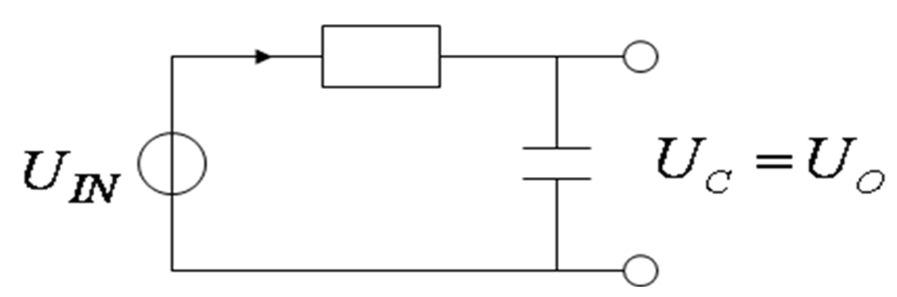
\includegraphics[width=0.7\linewidth]{Lab3_RC_Network}
\caption{An RC network is a classical example of a First Order System.}
\label{fig:Lab3_RC_Network}
\end{figure}
 
This system can be described using a First Order differential equation as follows:

\begin{equation} \label{Eqn:StepResponseFirstOrderSystem1}
U_{IN} = \tau \dot{U}_{OUT} + U_{OUT}
\end{equation}
 

Translating this system to the Laplace domain using the definition 
\begin{equation} \label{Eqn:StepResponseFirstOrderSystem2}
L(f(t)) = \int_{t=0}^{t = \infty} f(t)e^{-st} dt
\end{equation}

gives:
\begin{equation} \label{Eqn:StepResponseFirstOrderSystem3}
U_{IN}(s) = \tau s U_{OUT}(s) + U_{OUT}(s)
\end{equation}

Therefore the transfer function can be written as:
\begin{equation} \label{Eqn:StepResponseFirstOrderSystem4}
\dfrac{U_{OUT}(s)}{U_{IN}(s)} = \dfrac{1}{\tau s + 1}
\end{equation}
 	 	
If we excite the system with a unit step function which has a Laplace Transform of $\dfrac{1}{s}$, the output $U_{OUT}(s)$  can be written as:
\begin{equation} \label{Eqn:StepResponseFirstOrderSystem5}
U_{OUT}(s) = \dfrac{1}{\tau s + 1}U_{IN}(s) = \dfrac{1}{\tau s + 1} \dfrac{1}{s}
\end{equation}

This can be transformed back to time using Partial Fraction Expansion and the Laplace Transform Table. The solution is as follows:
\begin{equation} \label{Eqn:StepResponseFirstOrderSystem6}
U_{OUT}(t) = 1 - e^{-\dfrac{t}{\tau}}
\end{equation}

Similarly if we excite the system with a pulse (Dirac delta distribution) with has a Laplace Transform of 1, the output $U_{OUT}(s)$ can be written as:
\begin{equation} \label{Eqn:StepResponseFirstOrderSystem7}
U_{OUT}(s) = \dfrac{1}{\tau s + 1}U_{IN}(s) = \dfrac{1}{\tau s + 1}
\end{equation}

This can be transformed back to time using Partial Fraction Expansion and the Laplace Transform Table. The solution is as follows:
\begin{equation} \label{Eqn:StepResponseFirstOrderSystem8}
U_{OUT}(t) = \dfrac{1}{\tau} e^{-\dfrac{t}{\tau}}
\end{equation}

\section{Equipment}

\begin{enumerate}
\item Power supply
\item Bread board
\item Capacitor, 1 $nF$
\item Resistor, 100k
\item Function generator
\item Oscilloscope
\end{enumerate}

\section{Procedures}

\begin{enumerate}
\item Construct the simple schematic shown in Figure \ref{fig:Lab3_RC_Network} using a resistor of 100k (tolerance 5\%) and a capacitor of 1 $nF$.
\item Measure the "exact" value of the resistor using a multimeter. 
\item Measure the "exact" value of the capacitor using a capacitance meter.
\item Calculate the value of the time constant $\tau = RC$.
\item Use the MatLab \textbf{step} function to simulate the system unit step response. If you need help type "help step" in the MatLab command prompt. \textbf{Paste the output in your lab report}.
\item Use the MatLab \textbf{impulse} function to compute the impulse response of the system. \textbf{Paste the output in your lab report}.
\item Use the generator to put a 1kHz block wave with a peak-peak value of 10V on the scope. Show the input in Channel 1, and the output in Channel 2.
\item Calculate the same RC time constant from measurements. How close is your measurement to the theoretical value?
\end{enumerate}

\section{Questions}

Q1: How can you tell from the differential equation that the unit of the time constant is second?\\
A1:\\

Q2: Show that the unit of R*C is indeed second using Ohm?s Law and the Capacitor Equation.\\
A2:\\

Q3: If you had the choice to measure either the step or impulse response, which one would you prefer and why?\\
A3:\\

Q4: If you put a square wave with an amplitude of 1 volt on an RC network as shown in \ref{fig:Lab3_RC_Network}, what is the value of the response at $t = \tau$ ?\\
A4:\\

\end{document}
